\documentclass[1p]{elsarticle_modified}
%\bibliographystyle{elsarticle-num}

%\usepackage[colorlinks]{hyperref}
%\usepackage{abbrmath_seonhwa} %\Abb, \Ascr, \Acal ,\Abf, \Afrak
\usepackage{amsfonts}
\usepackage{amssymb}
\usepackage{amsmath}
\usepackage{amsthm}
\usepackage{scalefnt}
\usepackage{amsbsy}
\usepackage{kotex}
\usepackage{caption}
\usepackage{subfig}
\usepackage{color}
\usepackage{graphicx}
\usepackage{xcolor} %% white, black, red, green, blue, cyan, magenta, yellow
\usepackage{float}
\usepackage{setspace}
\usepackage{hyperref}

\usepackage{tikz}
\usetikzlibrary{arrows}

\usepackage{multirow}
\usepackage{array} % fixed length table
\usepackage{hhline}

%%%%%%%%%%%%%%%%%%%%%
\makeatletter
\renewcommand*\env@matrix[1][\arraystretch]{%
	\edef\arraystretch{#1}%
	\hskip -\arraycolsep
	\let\@ifnextchar\new@ifnextchar
	\array{*\c@MaxMatrixCols c}}
\makeatother %https://tex.stackexchange.com/questions/14071/how-can-i-increase-the-line-spacing-in-a-matrix
%%%%%%%%%%%%%%%

\usepackage[normalem]{ulem}

\newcommand{\msout}[1]{\ifmmode\text{\sout{\ensuremath{#1}}}\else\sout{#1}\fi}
%SOURCE: \msout is \stkout macro in https://tex.stackexchange.com/questions/20609/strikeout-in-math-mode

\newcommand{\cancel}[1]{
	\ifmmode
	{\color{red}\msout{#1}}
	\else
	{\color{red}\sout{#1}}
	\fi
}

\newcommand{\add}[1]{
	{\color{blue}\uwave{#1}}
}

\newcommand{\replace}[2]{
	\ifmmode
	{\color{red}\msout{#1}}{\color{blue}\uwave{#2}}
	\else
	{\color{red}\sout{#1}}{\color{blue}\uwave{#2}}
	\fi
}

\newcommand{\Sol}{\mathcal{S}} %segment
\newcommand{\D}{D} %diagram
\newcommand{\A}{\mathcal{A}} %arc


%%%%%%%%%%%%%%%%%%%%%%%%%%%%%5 test

\def\sl{\operatorname{\textup{SL}}(2,\Cbb)}
\def\psl{\operatorname{\textup{PSL}}(2,\Cbb)}
\def\quan{\mkern 1mu \triangleright \mkern 1mu}

\theoremstyle{definition}
\newtheorem{thm}{Theorem}[section]
\newtheorem{prop}[thm]{Proposition}
\newtheorem{lem}[thm]{Lemma}
\newtheorem{ques}[thm]{Question}
\newtheorem{cor}[thm]{Corollary}
\newtheorem{defn}[thm]{Definition}
\newtheorem{exam}[thm]{Example}
\newtheorem{rmk}[thm]{Remark}
\newtheorem{alg}[thm]{Algorithm}

\newcommand{\I}{\sqrt{-1}}
\begin{document}

%\begin{frontmatter}
%
%\title{Boundary parabolic representations of knots up to 8 crossings}
%
%%% Group authors per affiliation:
%\author{Yunhi Cho} 
%\address{Department of Mathematics, University of Seoul, Seoul, Korea}
%\ead{yhcho@uos.ac.kr}
%
%
%\author{Seonhwa Kim} %\fnref{s_kim}}
%\address{Center for Geometry and Physics, Institute for Basic Science, Pohang, 37673, Korea}
%\ead{ryeona17@ibs.re.kr}
%
%\author{Hyuk Kim}
%\address{Department of Mathematical Sciences, Seoul National University, Seoul 08826, Korea}
%\ead{hyukkim@snu.ac.kr}
%
%\author{Seokbeom Yoon}
%\address{Department of Mathematical Sciences, Seoul National University, Seoul, 08826,  Korea}
%\ead{sbyoon15@snu.ac.kr}
%
%\begin{abstract}
%We find all boundary parabolic representation of knots up to 8 crossings.
%
%\end{abstract}
%\begin{keyword}
%    \MSC[2010] 57M25 
%\end{keyword}
%
%\end{frontmatter}

%\linenumbers
%\tableofcontents
%
\newcommand\colored[1]{\textcolor{white}{\rule[-0.35ex]{0.8em}{1.4ex}}\kern-0.8em\color{red} #1}%
%\newcommand\colored[1]{\textcolor{white}{ #1}\kern-2.17ex	\textcolor{white}{ #1}\kern-1.81ex	\textcolor{white}{ #1}\kern-2.15ex\color{red}#1	}

{\Large $\underline{12n_{0718}~(K12n_{0718})}$}

\setlength{\tabcolsep}{10pt}
\renewcommand{\arraystretch}{1.6}
\vspace{1cm}\begin{tabular}{m{100pt}>{\centering\arraybackslash}m{274pt}}
\multirow{5}{120pt}{
	\centering
	\includegraphics[width=112pt]{../../../GIT/diagram.site/Diagrams/png/2807_12n_0718.png}\\
\ \ \ A knot diagram\footnotemark}&
\allowdisplaybreaks
\textbf{Linearized knot diagam} \\
\cline{2-2}
 &
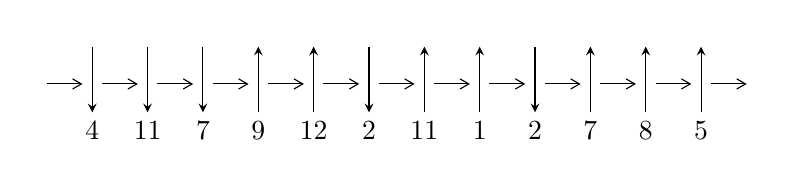
\begin{tikzpicture}[x=20pt, y=17pt]
	% nodes
	\node (C0) at (0, 0) {};
	\node (C1) at (1, 0) {};
	\node (C1U) at (1, +1) {};
	\node (C1D) at (1, -1) {4};

	\node (C2) at (2, 0) {};
	\node (C2U) at (2, +1) {};
	\node (C2D) at (2, -1) {11};

	\node (C3) at (3, 0) {};
	\node (C3U) at (3, +1) {};
	\node (C3D) at (3, -1) {7};

	\node (C4) at (4, 0) {};
	\node (C4U) at (4, +1) {};
	\node (C4D) at (4, -1) {9};

	\node (C5) at (5, 0) {};
	\node (C5U) at (5, +1) {};
	\node (C5D) at (5, -1) {12};

	\node (C6) at (6, 0) {};
	\node (C6U) at (6, +1) {};
	\node (C6D) at (6, -1) {2};

	\node (C7) at (7, 0) {};
	\node (C7U) at (7, +1) {};
	\node (C7D) at (7, -1) {11};

	\node (C8) at (8, 0) {};
	\node (C8U) at (8, +1) {};
	\node (C8D) at (8, -1) {1};

	\node (C9) at (9, 0) {};
	\node (C9U) at (9, +1) {};
	\node (C9D) at (9, -1) {2};

	\node (C10) at (10, 0) {};
	\node (C10U) at (10, +1) {};
	\node (C10D) at (10, -1) {7};

	\node (C11) at (11, 0) {};
	\node (C11U) at (11, +1) {};
	\node (C11D) at (11, -1) {8};

	\node (C12) at (12, 0) {};
	\node (C12U) at (12, +1) {};
	\node (C12D) at (12, -1) {5};
	\node (C13) at (13, 0) {};

	% arrows
	\draw[->,>={angle 60}]
	(C0) edge (C1) (C1) edge (C2) (C2) edge (C3) (C3) edge (C4) (C4) edge (C5) (C5) edge (C6) (C6) edge (C7) (C7) edge (C8) (C8) edge (C9) (C9) edge (C10) (C10) edge (C11) (C11) edge (C12) (C12) edge (C13) ;	\draw[->,>=stealth]
	(C1U) edge (C1D) (C2U) edge (C2D) (C3U) edge (C3D) (C4D) edge (C4U) (C5D) edge (C5U) (C6U) edge (C6D) (C7D) edge (C7U) (C8D) edge (C8U) (C9U) edge (C9D) (C10D) edge (C10U) (C11D) edge (C11U) (C12D) edge (C12U) ;
	\end{tikzpicture} \\
\hhline{~~} \\& 
\textbf{Solving Sequence} \\ \cline{2-2} 
 &
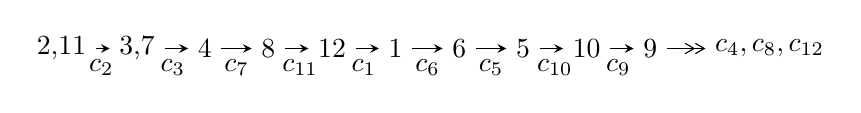
\begin{tikzpicture}[x=23pt, y=7pt]
	% node
	\node (A0) at (-1/8, 0) {2,11};
	\node (A1) at (17/16, 0) {3,7};
	\node (A2) at (17/8, 0) {4};
	\node (A3) at (25/8, 0) {8};
	\node (A4) at (33/8, 0) {12};
	\node (A5) at (41/8, 0) {1};
	\node (A6) at (49/8, 0) {6};
	\node (A7) at (57/8, 0) {5};
	\node (A8) at (65/8, 0) {10};
	\node (A9) at (73/8, 0) {9};
	\node (C1) at (1/2, -1) {$c_{2}$};
	\node (C2) at (13/8, -1) {$c_{3}$};
	\node (C3) at (21/8, -1) {$c_{7}$};
	\node (C4) at (29/8, -1) {$c_{11}$};
	\node (C5) at (37/8, -1) {$c_{1}$};
	\node (C6) at (45/8, -1) {$c_{6}$};
	\node (C7) at (53/8, -1) {$c_{5}$};
	\node (C8) at (61/8, -1) {$c_{10}$};
	\node (C9) at (69/8, -1) {$c_{9}$};
	\node (A10) at (11, 0) {$c_{4},c_{8},c_{12}$};

	% edge
	\draw[->,>=stealth]	
	(A0) edge (A1) (A1) edge (A2) (A2) edge (A3) (A3) edge (A4) (A4) edge (A5) (A5) edge (A6) (A6) edge (A7) (A7) edge (A8) (A8) edge (A9) ;
	\draw[->>,>={angle 60}]	
	(A9) edge (A10);
\end{tikzpicture} \\ 

\end{tabular} \\

\footnotetext{
The image of knot diagram is generated by the software ``\textbf{Draw programme}" developed by Andrew Bartholomew(\url{http://www.layer8.co.uk/maths/draw/index.htm\#Running-draw}), where we modified some parts for our purpose(\url{https://github.com/CATsTAILs/LinksPainter}).
}\phantom \\ \newline 
\centering \textbf{Ideals for irreducible components\footnotemark of $X_{\text{par}}$} 
 
\begin{align*}
I^u_{1}&=\langle 
13 u^5-14 u^4+83 u^3-84 u^2+67 b-74 u-31,\;-24 u^5+31 u^4-179 u^3+186 u^2+67 a+49 u+16,\\
\phantom{I^u_{1}}&\phantom{= \langle  }u^6+8 u^4+2 u^3+4 u^2+u+1\rangle \\
I^u_{2}&=\langle 
-1569393106 u^{14}-7670004252 u^{13}+\cdots+10430913127 b-4860457910,\\
\phantom{I^u_{2}}&\phantom{= \langle  }20548723543 u^{14}+25409181453 u^{13}+\cdots+10430913127 a-34629938205,\\
\phantom{I^u_{2}}&\phantom{= \langle  }u^{15}+u^{14}+16 u^{13}+15 u^{12}+67 u^{11}+68 u^{10}-6 u^9+55 u^8-21 u^7+47 u^6-22 u^5+20 u^4-7 u^3+6 u^2-2 u+1\rangle \\
I^u_{3}&=\langle 
53383992 u^{13}-54254216 u^{12}+\cdots+162743197 b+4010822,\\
\phantom{I^u_{3}}&\phantom{= \langle  }-157493798 u^{13}+153482976 u^{12}+\cdots+162743197 a-113034563,\\
\phantom{I^u_{3}}&\phantom{= \langle  }u^{14}- u^{13}+2 u^{12}- u^{11}-23 u^{10}+20 u^9+63 u^8-19 u^7-48 u^6+20 u^5+26 u^4-6 u^3-5 u^2+u+1\rangle \\
I^u_{4}&=\langle 
-1.12905\times10^{44} u^{23}-4.55305\times10^{43} u^{22}+\cdots+2.57192\times10^{47} b-2.14246\times10^{47},\\
\phantom{I^u_{4}}&\phantom{= \langle  }6.26307\times10^{45} u^{23}+9.22804\times10^{44} u^{22}+\cdots+5.24028\times10^{48} a-1.07233\times10^{49},\\
\phantom{I^u_{4}}&\phantom{= \langle  }u^{24}+23 u^{22}+\cdots-507 u+163\rangle \\
I^u_{5}&=\langle 
b+u-1,\;a- u+1,\;u^2- u+1\rangle \\
I^u_{6}&=\langle 
b^2- b+1,\;a-1,\;u+1\rangle \\
\\
\end{align*}
\raggedright * 6 irreducible components of $\dim_{\mathbb{C}}=0$, with total 63 representations.\\
\footnotetext{All coefficients of polynomials are rational numbers. But the coefficients are sometimes approximated in decimal forms when there is not enough margin.}
\newpage
\renewcommand{\arraystretch}{1}
\centering \section*{I. $I^u_{1}= \langle 13 u^5-14 u^4+\cdots+67 b-31,\;-24 u^5+31 u^4+\cdots+67 a+16,\;u^6+8 u^4+2 u^3+4 u^2+u+1 \rangle$}
\flushleft \textbf{(i) Arc colorings}\\
\begin{tabular}{m{7pt} m{180pt} m{7pt} m{180pt} }
\flushright $a_{2}=$&$\begin{pmatrix}1\\0\end{pmatrix}$ \\
\flushright $a_{11}=$&$\begin{pmatrix}0\\u\end{pmatrix}$ \\
\flushright $a_{3}=$&$\begin{pmatrix}1\\u^2\end{pmatrix}$ \\
\flushright $a_{7}=$&$\begin{pmatrix}0.358209 u^{5}-0.462687 u^{4}+\cdots-0.731343 u-0.238806\\-0.194030 u^{5}+0.208955 u^{4}+\cdots+1.10448 u+0.462687\end{pmatrix}$ \\
\flushright $a_{4}=$&$\begin{pmatrix}-0.462687 u^{5}-0.194030 u^{4}+\cdots-0.597015 u+0.641791\\0.208955 u^{5}+0.313433 u^{4}+\cdots+0.656716 u+0.194030\end{pmatrix}$ \\
\flushright $a_{8}=$&$\begin{pmatrix}0.358209 u^{5}-0.462687 u^{4}+\cdots-0.731343 u-0.238806\\u\end{pmatrix}$ \\
\flushright $a_{12}=$&$\begin{pmatrix}-0.208955 u^{5}-0.313433 u^{4}+\cdots-1.65672 u-1.19403\\-0.194030 u^{5}+0.208955 u^{4}+\cdots+1.10448 u+0.462687\end{pmatrix}$ \\
\flushright $a_{1}=$&$\begin{pmatrix}-0.671642 u^{5}-0.507463 u^{4}+\cdots-2.25373 u+0.447761\\0.268657 u^{5}+0.402985 u^{4}+\cdots+1.70149 u+0.820896\end{pmatrix}$ \\
\flushright $a_{6}=$&$\begin{pmatrix}0.164179 u^{5}-0.253731 u^{4}+\cdots+0.373134 u+0.223881\\-0.194030 u^{5}+0.208955 u^{4}+\cdots+1.10448 u+0.462687\end{pmatrix}$ \\
\flushright $a_{5}=$&$\begin{pmatrix}-0.402985 u^{5}-0.104478 u^{4}+\cdots+0.447761 u+1.26866\\0.522388 u^{5}+0.283582 u^{4}+\cdots+1.64179 u-0.0149254\end{pmatrix}$ \\
\flushright $a_{10}=$&$\begin{pmatrix}0.208955 u^{5}+0.313433 u^{4}+\cdots+1.65672 u+1.19403\\0.164179 u^{5}-0.253731 u^{4}+\cdots+0.373134 u-0.776119\end{pmatrix}$ \\
\flushright $a_{9}=$&$\begin{pmatrix}0.373134 u^{5}+0.0597015 u^{4}+\cdots+2.02985 u+0.417910\\0.164179 u^{5}-0.253731 u^{4}+\cdots+0.373134 u-0.776119\end{pmatrix}$\\&\end{tabular}
\flushleft \textbf{(ii) Obstruction class $= -1$}\\~\\
\flushleft \textbf{(iii) Cusp Shapes $= \frac{193}{67} u^5+\frac{122}{67} u^4+\frac{1526}{67} u^3+\frac{1335}{67} u^2+\frac{999}{67} u+\frac{720}{67}$}\\~\\
\newpage\renewcommand{\arraystretch}{1}
\flushleft \textbf{(iv) u-Polynomials at the component}\newline \\
\begin{tabular}{m{50pt}|m{274pt}}
Crossings & \hspace{64pt}u-Polynomials at each crossing \\
\hline $$\begin{aligned}c_{1}\end{aligned}$$&$\begin{aligned}
&u^6-4 u^5+9 u^4-11 u^3+8 u^2-3 u+1
\end{aligned}$\\
\hline $$\begin{aligned}c_{2},c_{3}\end{aligned}$$&$\begin{aligned}
&u^6+8 u^4-2 u^3+4 u^2- u+1
\end{aligned}$\\
\hline $$\begin{aligned}c_{4},c_{8}\end{aligned}$$&$\begin{aligned}
&u^6-2 u^3+4 u^2-3 u+1
\end{aligned}$\\
\hline $$\begin{aligned}c_{5},c_{12}\end{aligned}$$&$\begin{aligned}
&(u^3-2 u^2+3 u-1)^2
\end{aligned}$\\
\hline $$\begin{aligned}c_{6}\end{aligned}$$&$\begin{aligned}
&u^6- u^5+7 u^4+8 u^2-5 u+1
\end{aligned}$\\
\hline $$\begin{aligned}c_{7},c_{10},c_{11}\end{aligned}$$&$\begin{aligned}
&u^6-3 u^5+5 u^3- u^2-2 u+1
\end{aligned}$\\
\hline $$\begin{aligned}c_{9}\end{aligned}$$&$\begin{aligned}
&u^6-5 u^5+13 u^4-16 u^3+12 u^2-5 u+1
\end{aligned}$\\
\hline
\end{tabular}\\~\\
\newpage\renewcommand{\arraystretch}{1}
\flushleft \textbf{(v) Riley Polynomials at the component}\newline \\
\begin{tabular}{m{50pt}|m{274pt}}
Crossings & \hspace{64pt}Riley Polynomials at each crossing \\
\hline $$\begin{aligned}c_{1}\end{aligned}$$&$\begin{aligned}
&y^6+2 y^5+9 y^4+y^3+16 y^2+7 y+1
\end{aligned}$\\
\hline $$\begin{aligned}c_{2},c_{3}\end{aligned}$$&$\begin{aligned}
&y^6+16 y^5+72 y^4+62 y^3+28 y^2+7 y+1
\end{aligned}$\\
\hline $$\begin{aligned}c_{4},c_{8}\end{aligned}$$&$\begin{aligned}
&y^6+8 y^4-2 y^3+4 y^2- y+1
\end{aligned}$\\
\hline $$\begin{aligned}c_{5},c_{12}\end{aligned}$$&$\begin{aligned}
&(y^3+2 y^2+5 y-1)^2
\end{aligned}$\\
\hline $$\begin{aligned}c_{6}\end{aligned}$$&$\begin{aligned}
&y^6+13 y^5+65 y^4+104 y^3+78 y^2-9 y+1
\end{aligned}$\\
\hline $$\begin{aligned}c_{7},c_{10},c_{11}\end{aligned}$$&$\begin{aligned}
&y^6-9 y^5+28 y^4-35 y^3+21 y^2-6 y+1
\end{aligned}$\\
\hline $$\begin{aligned}c_{9}\end{aligned}$$&$\begin{aligned}
&y^6+y^5+33 y^4+8 y^3+10 y^2- y+1
\end{aligned}$\\
\hline
\end{tabular}\\~\\
\newpage\flushleft \textbf{(vi) Complex Volumes and Cusp Shapes}
$$\begin{array}{c|c|c}  
\text{Solutions to }I^u_{1}& \I (\text{vol} + \sqrt{-1}CS) & \text{Cusp shape}\\
 \hline 
\begin{aligned}
u &= \phantom{-}0.175218 + 0.614017 I \\
a &= \phantom{-}0.08270 - 1.43799 I \\
b &= \phantom{-}0.455994 + 1.129810 I\end{aligned}
 & \phantom{-}1.18623 - 4.16039 I & \phantom{-}2.50198 + 9.24184 I \\ \hline\begin{aligned}
u &= \phantom{-}0.175218 - 0.614017 I \\
a &= \phantom{-}0.08270 + 1.43799 I \\
b &= \phantom{-}0.455994 - 1.129810 I\end{aligned}
 & \phantom{-}1.18623 + 4.16039 I & \phantom{-}2.50198 - 9.24184 I \\ \hline\begin{aligned}
u &= -0.307599 + 0.479689 I \\
a &= \phantom{-}0.877439 + 0.479689 I \\
b &= -0.284920 + 0.155763 I\end{aligned}
 & \phantom{-}1.134710 - 0.529643 I & \phantom{-}7.45884 + 1.83935 I \\ \hline\begin{aligned}
u &= -0.307599 - 0.479689 I \\
a &= \phantom{-}0.877439 - 0.479689 I \\
b &= -0.284920 - 0.155763 I\end{aligned}
 & \phantom{-}1.134710 + 0.529643 I & \phantom{-}7.45884 - 1.83935 I \\ \hline\begin{aligned}
u &= \phantom{-}0.13238 + 2.74513 I \\
a &= \phantom{-}0.039862 + 0.693124 I \\
b &= -0.67107 - 2.43695 I\end{aligned}
 & \phantom{-}14.1284 - 13.7510 I & \phantom{-}4.53918 + 6.26128 I \\ \hline\begin{aligned}
u &= \phantom{-}0.13238 - 2.74513 I \\
a &= \phantom{-}0.039862 - 0.693124 I \\
b &= -0.67107 + 2.43695 I\end{aligned}
 & \phantom{-}14.1284 + 13.7510 I & \phantom{-}4.53918 - 6.26128 I\\
 \hline 
 \end{array}$$\newpage\newpage\renewcommand{\arraystretch}{1}
\centering \section*{II. $I^u_{2}= \langle -1.57\times10^{9} u^{14}-7.67\times10^{9} u^{13}+\cdots+1.04\times10^{10} b-4.86\times10^{9},\;2.05\times10^{10} u^{14}+2.54\times10^{10} u^{13}+\cdots+1.04\times10^{10} a-3.46\times10^{10},\;u^{15}+u^{14}+\cdots-2 u+1 \rangle$}
\flushleft \textbf{(i) Arc colorings}\\
\begin{tabular}{m{7pt} m{180pt} m{7pt} m{180pt} }
\flushright $a_{2}=$&$\begin{pmatrix}1\\0\end{pmatrix}$ \\
\flushright $a_{11}=$&$\begin{pmatrix}0\\u\end{pmatrix}$ \\
\flushright $a_{3}=$&$\begin{pmatrix}1\\u^2\end{pmatrix}$ \\
\flushright $a_{7}=$&$\begin{pmatrix}-1.96998 u^{14}-2.43595 u^{13}+\cdots-8.60582 u+3.31993\\0.150456 u^{14}+0.735315 u^{13}+\cdots+2.03805 u+0.465967\end{pmatrix}$ \\
\flushright $a_{4}=$&$\begin{pmatrix}-0.465967 u^{14}-0.315511 u^{13}+\cdots-0.620033 u+2.96998\\0.584859 u^{14}+0.726095 u^{13}+\cdots+0.766879 u-0.150456\end{pmatrix}$ \\
\flushright $a_{8}=$&$\begin{pmatrix}-1.96998 u^{14}-2.43595 u^{13}+\cdots-8.60582 u+3.31993\\u\end{pmatrix}$ \\
\flushright $a_{12}=$&$\begin{pmatrix}-1.55974 u^{14}-0.980765 u^{13}+\cdots-5.08122 u+3.74389\\0.150456 u^{14}+0.735315 u^{13}+\cdots+2.03805 u+0.465967\end{pmatrix}$ \\
\flushright $a_{1}=$&$\begin{pmatrix}-2.12527 u^{14}-2.81645 u^{13}+\cdots-2.52477 u+1.85292\\0.665898 u^{14}+0.835107 u^{13}+\cdots+1.04529 u+0.832419\end{pmatrix}$ \\
\flushright $a_{6}=$&$\begin{pmatrix}-1.81953 u^{14}-1.70064 u^{13}+\cdots-6.56777 u+3.78590\\0.150456 u^{14}+0.735315 u^{13}+\cdots+2.03805 u+0.465967\end{pmatrix}$ \\
\flushright $a_{5}=$&$\begin{pmatrix}-2.60944 u^{14}-4.20613 u^{13}+\cdots-7.32190 u+1.21409\\-0.774010 u^{14}-0.545592 u^{13}+\cdots-2.36170 u+2.98355\end{pmatrix}$ \\
\flushright $a_{10}=$&$\begin{pmatrix}1.55974 u^{14}+0.980765 u^{13}+\cdots+5.08122 u-3.74389\\-0.552009 u^{14}-1.50756 u^{13}+\cdots-2.75574 u+0.113009\end{pmatrix}$ \\
\flushright $a_{9}=$&$\begin{pmatrix}1.00773 u^{14}-0.526796 u^{13}+\cdots+2.32548 u-3.63089\\-0.552009 u^{14}-1.50756 u^{13}+\cdots-2.75574 u+0.113009\end{pmatrix}$\\&\end{tabular}
\flushleft \textbf{(ii) Obstruction class $= -1$}\\~\\
\flushleft \textbf{(iii) Cusp Shapes $= -\frac{61025071082}{10430913127} u^{14}-\frac{87492839805}{10430913127} u^{13}+\cdots-\frac{60233840046}{10430913127} u+\frac{63546445223}{10430913127}$}\\~\\
\newpage\renewcommand{\arraystretch}{1}
\flushleft \textbf{(iv) u-Polynomials at the component}\newline \\
\begin{tabular}{m{50pt}|m{274pt}}
Crossings & \hspace{64pt}u-Polynomials at each crossing \\
\hline $$\begin{aligned}c_{1}\end{aligned}$$&$\begin{aligned}
&u^{15}-8 u^{14}+\cdots-26 u+4
\end{aligned}$\\
\hline $$\begin{aligned}c_{2},c_{3}\end{aligned}$$&$\begin{aligned}
&u^{15}- u^{14}+\cdots-2 u-1
\end{aligned}$\\
\hline $$\begin{aligned}c_{4},c_{8}\end{aligned}$$&$\begin{aligned}
&u^{15}+u^{12}+\cdots+6 u^2-1
\end{aligned}$\\
\hline $$\begin{aligned}c_{5},c_{12}\end{aligned}$$&$\begin{aligned}
&u^{15}-8 u^{14}+\cdots-128 u+32
\end{aligned}$\\
\hline $$\begin{aligned}c_{6}\end{aligned}$$&$\begin{aligned}
&u^{15}+4 u^{14}+\cdots+14 u+1
\end{aligned}$\\
\hline $$\begin{aligned}c_{7},c_{10},c_{11}\end{aligned}$$&$\begin{aligned}
&u^{15}-6 u^{14}+\cdots+28 u-16
\end{aligned}$\\
\hline $$\begin{aligned}c_{9}\end{aligned}$$&$\begin{aligned}
&u^{15}+4 u^{14}+\cdots-18 u-9
\end{aligned}$\\
\hline
\end{tabular}\\~\\
\newpage\renewcommand{\arraystretch}{1}
\flushleft \textbf{(v) Riley Polynomials at the component}\newline \\
\begin{tabular}{m{50pt}|m{274pt}}
Crossings & \hspace{64pt}Riley Polynomials at each crossing \\
\hline $$\begin{aligned}c_{1}\end{aligned}$$&$\begin{aligned}
&y^{15}+2 y^{13}+\cdots-68 y-16
\end{aligned}$\\
\hline $$\begin{aligned}c_{2},c_{3}\end{aligned}$$&$\begin{aligned}
&y^{15}+31 y^{14}+\cdots-8 y-1
\end{aligned}$\\
\hline $$\begin{aligned}c_{4},c_{8}\end{aligned}$$&$\begin{aligned}
&y^{15}+12 y^{13}+\cdots+12 y-1
\end{aligned}$\\
\hline $$\begin{aligned}c_{5},c_{12}\end{aligned}$$&$\begin{aligned}
&y^{15}+2 y^{14}+\cdots-3584 y-1024
\end{aligned}$\\
\hline $$\begin{aligned}c_{6}\end{aligned}$$&$\begin{aligned}
&y^{15}+26 y^{14}+\cdots+34 y-1
\end{aligned}$\\
\hline $$\begin{aligned}c_{7},c_{10},c_{11}\end{aligned}$$&$\begin{aligned}
&y^{15}-20 y^{14}+\cdots-1232 y-256
\end{aligned}$\\
\hline $$\begin{aligned}c_{9}\end{aligned}$$&$\begin{aligned}
&y^{15}+14 y^{14}+\cdots-288 y-81
\end{aligned}$\\
\hline
\end{tabular}\\~\\
\newpage\flushleft \textbf{(vi) Complex Volumes and Cusp Shapes}
$$\begin{array}{c|c|c}  
\text{Solutions to }I^u_{2}& \I (\text{vol} + \sqrt{-1}CS) & \text{Cusp shape}\\
 \hline 
\begin{aligned}
u &= -0.358852 + 0.655382 I \\
a &= \phantom{-}0.37132 + 1.53080 I \\
b &= \phantom{-}0.249515 + 0.020338 I\end{aligned}
 & \phantom{-}0.647850 + 0.593610 I & \phantom{-}0.397147 - 0.414996 I \\ \hline\begin{aligned}
u &= -0.358852 - 0.655382 I \\
a &= \phantom{-}0.37132 - 1.53080 I \\
b &= \phantom{-}0.249515 - 0.020338 I\end{aligned}
 & \phantom{-}0.647850 - 0.593610 I & \phantom{-}0.397147 + 0.414996 I \\ \hline\begin{aligned}
u &= -0.362442 + 0.521099 I \\
a &= -1.62550 - 1.14103 I \\
b &= -0.565588 + 1.295060 I\end{aligned}
 & \phantom{-}6.17652 - 3.16479 I & \phantom{-}8.46791 + 3.96283 I \\ \hline\begin{aligned}
u &= -0.362442 - 0.521099 I \\
a &= -1.62550 + 1.14103 I \\
b &= -0.565588 - 1.295060 I\end{aligned}
 & \phantom{-}6.17652 + 3.16479 I & \phantom{-}8.46791 - 3.96283 I \\ \hline\begin{aligned}
u &= \phantom{-}0.495956 + 0.351454 I \\
a &= \phantom{-}0.594839 + 0.597610 I \\
b &= \phantom{-}0.360462 + 0.632001 I\end{aligned}
 & -1.23951 - 1.59759 I & -0.60489 + 4.37134 I \\ \hline\begin{aligned}
u &= \phantom{-}0.495956 - 0.351454 I \\
a &= \phantom{-}0.594839 - 0.597610 I \\
b &= \phantom{-}0.360462 - 0.632001 I\end{aligned}
 & -1.23951 + 1.59759 I & -0.60489 - 4.37134 I \\ \hline\begin{aligned}
u &= \phantom{-}0.177403 + 0.564115 I \\
a &= -1.56471 - 0.13961 I \\
b &= \phantom{-}0.654033 + 0.290971 I\end{aligned}
 & -2.12993 + 3.66119 I & \phantom{-}1.84247 - 2.75515 I \\ \hline\begin{aligned}
u &= \phantom{-}0.177403 - 0.564115 I \\
a &= -1.56471 + 0.13961 I \\
b &= \phantom{-}0.654033 - 0.290971 I\end{aligned}
 & -2.12993 - 3.66119 I & \phantom{-}1.84247 + 2.75515 I \\ \hline\begin{aligned}
u &= \phantom{-}0.361509 + 0.466401 I \\
a &= \phantom{-}2.32217 - 1.05813 I \\
b &= \phantom{-}0.51667 + 1.34137 I\end{aligned}
 & \phantom{-}2.58286 + 9.32736 I & \phantom{-}5.11705 - 6.33212 I \\ \hline\begin{aligned}
u &= \phantom{-}0.361509 - 0.466401 I \\
a &= \phantom{-}2.32217 + 1.05813 I \\
b &= \phantom{-}0.51667 - 1.34137 I\end{aligned}
 & \phantom{-}2.58286 - 9.32736 I & \phantom{-}5.11705 + 6.33212 I\\
 \hline 
 \end{array}$$\newpage$$\begin{array}{c|c|c}  
\text{Solutions to }I^u_{2}& \I (\text{vol} + \sqrt{-1}CS) & \text{Cusp shape}\\
 \hline 
\begin{aligned}
u &= -1.47475\phantom{ +0.000000I} \\
a &= \phantom{-}0.909455\phantom{ +0.000000I} \\
b &= \phantom{-}0.503214\phantom{ +0.000000I}\end{aligned}
 & \phantom{-}2.65817\phantom{ +0.000000I} & \phantom{-}1.30990\phantom{ +0.000000I} \\ \hline\begin{aligned}
u &= \phantom{-}0.30799 + 2.79469 I \\
a &= -0.133260 + 0.638046 I \\
b &= \phantom{-}0.23778 - 2.35751 I\end{aligned}
 & \phantom{-}16.9670 + 6.2281 I & \phantom{-}6.62700 - 4.47239 I \\ \hline\begin{aligned}
u &= \phantom{-}0.30799 - 2.79469 I \\
a &= -0.133260 - 0.638046 I \\
b &= \phantom{-}0.23778 + 2.35751 I\end{aligned}
 & \phantom{-}16.9670 - 6.2281 I & \phantom{-}6.62700 + 4.47239 I \\ \hline\begin{aligned}
u &= -0.38419 + 2.88575 I \\
a &= \phantom{-}0.080416 + 0.603207 I \\
b &= \phantom{-}0.29553 - 2.22676 I\end{aligned}
 & \phantom{-}11.03220 + 4.65884 I & \phantom{-}2.00000 - 4.62633 I \\ \hline\begin{aligned}
u &= -0.38419 - 2.88575 I \\
a &= \phantom{-}0.080416 - 0.603207 I \\
b &= \phantom{-}0.29553 + 2.22676 I\end{aligned}
 & \phantom{-}11.03220 - 4.65884 I & \phantom{-}2.00000 + 4.62633 I\\
 \hline 
 \end{array}$$\newpage\newpage\renewcommand{\arraystretch}{1}
\centering \section*{III. $I^u_{3}= \langle 5.34\times10^{7} u^{13}-5.43\times10^{7} u^{12}+\cdots+1.63\times10^{8} b+4.01\times10^{6},\;-1.57\times10^{8} u^{13}+1.53\times10^{8} u^{12}+\cdots+1.63\times10^{8} a-1.13\times10^{8},\;u^{14}- u^{13}+\cdots+u+1 \rangle$}
\flushleft \textbf{(i) Arc colorings}\\
\begin{tabular}{m{7pt} m{180pt} m{7pt} m{180pt} }
\flushright $a_{2}=$&$\begin{pmatrix}1\\0\end{pmatrix}$ \\
\flushright $a_{11}=$&$\begin{pmatrix}0\\u\end{pmatrix}$ \\
\flushright $a_{3}=$&$\begin{pmatrix}1\\u^2\end{pmatrix}$ \\
\flushright $a_{7}=$&$\begin{pmatrix}0.967744 u^{13}-0.943099 u^{12}+\cdots-7.60104 u+0.694558\\-0.328026 u^{13}+0.333373 u^{12}+\cdots-1.99239 u-0.0246451\end{pmatrix}$ \\
\flushright $a_{4}=$&$\begin{pmatrix}-0.0246451 u^{13}+0.352671 u^{12}+\cdots+0.273186 u+1.96774\\-0.00534722 u^{13}+0.173641 u^{12}+\cdots-0.303381 u-0.328026\end{pmatrix}$ \\
\flushright $a_{8}=$&$\begin{pmatrix}0.967744 u^{13}-0.943099 u^{12}+\cdots-7.60104 u+0.694558\\- u\end{pmatrix}$ \\
\flushright $a_{12}=$&$\begin{pmatrix}-1.00142 u^{13}+1.17112 u^{12}+\cdots+10.0376 u-0.867819\\0.328026 u^{13}-0.333373 u^{12}+\cdots+1.99239 u+0.0246451\end{pmatrix}$ \\
\flushright $a_{1}=$&$\begin{pmatrix}-0.115338 u^{13}-0.488695 u^{12}+\cdots+1.49454 u+2.39877\\0.127699 u^{13}-0.330520 u^{12}+\cdots+0.882317 u+0.772326\end{pmatrix}$ \\
\flushright $a_{6}=$&$\begin{pmatrix}0.639718 u^{13}-0.609726 u^{12}+\cdots-9.59343 u+0.669913\\-0.328026 u^{13}+0.333373 u^{12}+\cdots-1.99239 u-0.0246451\end{pmatrix}$ \\
\flushright $a_{5}=$&$\begin{pmatrix}0.495091 u^{13}+0.698721 u^{12}+\cdots-12.6713 u-2.60480\\-0.333373 u^{13}+0.507014 u^{12}+\cdots-2.29577 u-1.35267\end{pmatrix}$ \\
\flushright $a_{10}=$&$\begin{pmatrix}1.00142 u^{13}-1.17112 u^{12}+\cdots-10.0376 u+0.867819\\-0.742720 u^{13}+0.616688 u^{12}+\cdots-0.824103 u+0.145057\end{pmatrix}$ \\
\flushright $a_{9}=$&$\begin{pmatrix}0.258696 u^{13}-0.554431 u^{12}+\cdots-10.8617 u+1.01288\\-0.742720 u^{13}+0.616688 u^{12}+\cdots-0.824103 u+0.145057\end{pmatrix}$\\&\end{tabular}
\flushleft \textbf{(ii) Obstruction class $= 1$}\\~\\
\flushleft \textbf{(iii) Cusp Shapes $= -\frac{585676500}{162743197} u^{13}+\frac{980281103}{162743197} u^{12}+\cdots+\frac{608482609}{162743197} u-\frac{380597444}{162743197}$}\\~\\
\newpage\renewcommand{\arraystretch}{1}
\flushleft \textbf{(iv) u-Polynomials at the component}\newline \\
\begin{tabular}{m{50pt}|m{274pt}}
Crossings & \hspace{64pt}u-Polynomials at each crossing \\
\hline $$\begin{aligned}c_{1}\end{aligned}$$&$\begin{aligned}
&u^{14}-9 u^{13}+\cdots-39 u+9
\end{aligned}$\\
\hline $$\begin{aligned}c_{2}\end{aligned}$$&$\begin{aligned}
&u^{14}- u^{13}+\cdots+u+1
\end{aligned}$\\
\hline $$\begin{aligned}c_{3}\end{aligned}$$&$\begin{aligned}
&u^{14}+u^{13}+\cdots- u+1
\end{aligned}$\\
\hline $$\begin{aligned}c_{4},c_{8}\end{aligned}$$&$\begin{aligned}
&u^{14}+2 u^{12}+\cdots- u+1
\end{aligned}$\\
\hline $$\begin{aligned}c_{5}\end{aligned}$$&$\begin{aligned}
&u^{14}+5 u^{13}+\cdots+4 u+5
\end{aligned}$\\
\hline $$\begin{aligned}c_{6}\end{aligned}$$&$\begin{aligned}
&u^{14}+u^{13}+\cdots- u+1
\end{aligned}$\\
\hline $$\begin{aligned}c_{7}\end{aligned}$$&$\begin{aligned}
&u^{14}-4 u^{13}+\cdots+4 u+1
\end{aligned}$\\
\hline $$\begin{aligned}c_{9}\end{aligned}$$&$\begin{aligned}
&u^{14}- u^{13}+\cdots+3 u+5
\end{aligned}$\\
\hline $$\begin{aligned}c_{10},c_{11}\end{aligned}$$&$\begin{aligned}
&u^{14}+4 u^{13}+\cdots-4 u+1
\end{aligned}$\\
\hline $$\begin{aligned}c_{12}\end{aligned}$$&$\begin{aligned}
&u^{14}-5 u^{13}+\cdots-4 u+5
\end{aligned}$\\
\hline
\end{tabular}\\~\\
\newpage\renewcommand{\arraystretch}{1}
\flushleft \textbf{(v) Riley Polynomials at the component}\newline \\
\begin{tabular}{m{50pt}|m{274pt}}
Crossings & \hspace{64pt}Riley Polynomials at each crossing \\
\hline $$\begin{aligned}c_{1}\end{aligned}$$&$\begin{aligned}
&y^{14}- y^{13}+\cdots+441 y+81
\end{aligned}$\\
\hline $$\begin{aligned}c_{2},c_{3}\end{aligned}$$&$\begin{aligned}
&y^{14}+3 y^{13}+\cdots-11 y+1
\end{aligned}$\\
\hline $$\begin{aligned}c_{4},c_{8}\end{aligned}$$&$\begin{aligned}
&y^{14}+4 y^{13}+\cdots+9 y+1
\end{aligned}$\\
\hline $$\begin{aligned}c_{5},c_{12}\end{aligned}$$&$\begin{aligned}
&y^{14}+5 y^{13}+\cdots+194 y+25
\end{aligned}$\\
\hline $$\begin{aligned}c_{6}\end{aligned}$$&$\begin{aligned}
&y^{14}+7 y^{13}+\cdots-9 y+1
\end{aligned}$\\
\hline $$\begin{aligned}c_{7},c_{10},c_{11}\end{aligned}$$&$\begin{aligned}
&y^{14}-20 y^{13}+\cdots+8 y+1
\end{aligned}$\\
\hline $$\begin{aligned}c_{9}\end{aligned}$$&$\begin{aligned}
&y^{14}+7 y^{13}+\cdots-159 y+25
\end{aligned}$\\
\hline
\end{tabular}\\~\\
\newpage\flushleft \textbf{(vi) Complex Volumes and Cusp Shapes}
$$\begin{array}{c|c|c}  
\text{Solutions to }I^u_{3}& \I (\text{vol} + \sqrt{-1}CS) & \text{Cusp shape}\\
 \hline 
\begin{aligned}
u &= -0.790557 + 0.311356 I \\
a &= \phantom{-}0.222610 - 0.126329 I \\
b &= \phantom{-}0.845913 - 0.487651 I\end{aligned}
 & -2.48510 + 1.52387 I & -12.05484 - 4.31807 I \\ \hline\begin{aligned}
u &= -0.790557 - 0.311356 I \\
a &= \phantom{-}0.222610 + 0.126329 I \\
b &= \phantom{-}0.845913 + 0.487651 I\end{aligned}
 & -2.48510 - 1.52387 I & -12.05484 + 4.31807 I \\ \hline\begin{aligned}
u &= \phantom{-}0.651265 + 0.441006 I \\
a &= \phantom{-}0.654355 + 0.591336 I \\
b &= -0.840663 + 0.070677 I\end{aligned}
 & -3.27577 - 5.02886 I & -3.36805 + 4.35249 I \\ \hline\begin{aligned}
u &= \phantom{-}0.651265 - 0.441006 I \\
a &= \phantom{-}0.654355 - 0.591336 I \\
b &= -0.840663 - 0.070677 I\end{aligned}
 & -3.27577 + 5.02886 I & -3.36805 - 4.35249 I \\ \hline\begin{aligned}
u &= -1.286040 + 0.174398 I \\
a &= -0.962915 - 0.327892 I \\
b &= -0.424318 - 0.274794 I\end{aligned}
 & \phantom{-}0.42007 + 8.20640 I & \phantom{-}2.95833 - 6.07795 I \\ \hline\begin{aligned}
u &= -1.286040 - 0.174398 I \\
a &= -0.962915 + 0.327892 I \\
b &= -0.424318 + 0.274794 I\end{aligned}
 & \phantom{-}0.42007 - 8.20640 I & \phantom{-}2.95833 + 6.07795 I \\ \hline\begin{aligned}
u &= \phantom{-}0.449003 + 0.276873 I \\
a &= -2.83110 + 0.52067 I \\
b &= -0.932191 - 0.915727 I\end{aligned}
 & \phantom{-}1.86269 - 0.47837 I & \phantom{-}4.00892 + 2.29799 I \\ \hline\begin{aligned}
u &= \phantom{-}0.449003 - 0.276873 I \\
a &= -2.83110 - 0.52067 I \\
b &= -0.932191 + 0.915727 I\end{aligned}
 & \phantom{-}1.86269 + 0.47837 I & \phantom{-}4.00892 - 2.29799 I \\ \hline\begin{aligned}
u &= -0.365580 + 0.259701 I \\
a &= \phantom{-}2.22502 + 1.59201 I \\
b &= \phantom{-}0.815180 - 0.576796 I\end{aligned}
 & \phantom{-}1.08385 + 2.12480 I & \phantom{-}2.10872 - 3.90851 I \\ \hline\begin{aligned}
u &= -0.365580 - 0.259701 I \\
a &= \phantom{-}2.22502 - 1.59201 I \\
b &= \phantom{-}0.815180 + 0.576796 I\end{aligned}
 & \phantom{-}1.08385 - 2.12480 I & \phantom{-}2.10872 + 3.90851 I\\
 \hline 
 \end{array}$$\newpage$$\begin{array}{c|c|c}  
\text{Solutions to }I^u_{3}& \I (\text{vol} + \sqrt{-1}CS) & \text{Cusp shape}\\
 \hline 
\begin{aligned}
u &= \phantom{-}1.75681 + 0.66656 I \\
a &= \phantom{-}0.711754 - 0.230141 I \\
b &= \phantom{-}0.662699 + 0.392339 I\end{aligned}
 & \phantom{-}2.71530 - 0.58653 I & -0.31767 + 11.02629 I \\ \hline\begin{aligned}
u &= \phantom{-}1.75681 - 0.66656 I \\
a &= \phantom{-}0.711754 + 0.230141 I \\
b &= \phantom{-}0.662699 - 0.392339 I\end{aligned}
 & \phantom{-}2.71530 + 0.58653 I & -0.31767 - 11.02629 I \\ \hline\begin{aligned}
u &= \phantom{-}0.08510 + 2.59262 I \\
a &= -0.019722 - 0.738947 I \\
b &= \phantom{-}0.37338 + 2.36028 I\end{aligned}
 & \phantom{-}14.4834 - 3.0320 I & \phantom{-}4.66457 + 0.35258 I \\ \hline\begin{aligned}
u &= \phantom{-}0.08510 - 2.59262 I \\
a &= -0.019722 + 0.738947 I \\
b &= \phantom{-}0.37338 - 2.36028 I\end{aligned}
 & \phantom{-}14.4834 + 3.0320 I & \phantom{-}4.66457 - 0.35258 I\\
 \hline 
 \end{array}$$\newpage\newpage\renewcommand{\arraystretch}{1}
\centering \section*{IV. $I^u_{4}= \langle -1.13\times10^{44} u^{23}-4.55\times10^{43} u^{22}+\cdots+2.57\times10^{47} b-2.14\times10^{47},\;6.26\times10^{45} u^{23}+9.23\times10^{44} u^{22}+\cdots+5.24\times10^{48} a-1.07\times10^{49},\;u^{24}+23 u^{22}+\cdots-507 u+163 \rangle$}
\flushleft \textbf{(i) Arc colorings}\\
\begin{tabular}{m{7pt} m{180pt} m{7pt} m{180pt} }
\flushright $a_{2}=$&$\begin{pmatrix}1\\0\end{pmatrix}$ \\
\flushright $a_{11}=$&$\begin{pmatrix}0\\u\end{pmatrix}$ \\
\flushright $a_{3}=$&$\begin{pmatrix}1\\u^2\end{pmatrix}$ \\
\flushright $a_{7}=$&$\begin{pmatrix}-0.00119518 u^{23}-0.000176098 u^{22}+\cdots-4.63707 u+2.04632\\0.000438993 u^{23}+0.000177030 u^{22}+\cdots+2.63368 u+0.833021\end{pmatrix}$ \\
\flushright $a_{4}=$&$\begin{pmatrix}-0.000916187 u^{23}-0.000184171 u^{22}+\cdots-0.122354 u+3.09669\\0.000590316 u^{23}+0.000590123 u^{22}+\cdots+4.74285 u+0.522808\end{pmatrix}$ \\
\flushright $a_{8}=$&$\begin{pmatrix}-0.00119518 u^{23}-0.000176098 u^{22}+\cdots-4.63707 u+2.04632\\0.000297902 u^{23}+0.0000128219 u^{22}+\cdots+2.52815 u+0.804317\end{pmatrix}$ \\
\flushright $a_{12}=$&$\begin{pmatrix}-0.000437714 u^{23}+0.000247445 u^{22}+\cdots+1.38888 u+0.570111\\-0.000184171 u^{23}+0.000425432 u^{22}+\cdots+2.63218 u+0.149338\end{pmatrix}$ \\
\flushright $a_{1}=$&$\begin{pmatrix}-0.00343719 u^{23}-0.000380507 u^{22}+\cdots-11.7851 u-1.62097\\-0.00160994 u^{23}-0.000560518 u^{22}+\cdots-7.70778 u+0.658868\end{pmatrix}$ \\
\flushright $a_{6}=$&$\begin{pmatrix}-0.000756187 u^{23}+9.31402\times10^{-7} u^{22}+\cdots-2.00339 u+2.87935\\0.000438993 u^{23}+0.000177030 u^{22}+\cdots+2.63368 u+0.833021\end{pmatrix}$ \\
\flushright $a_{5}=$&$\begin{pmatrix}0.00118185 u^{23}-0.000522705 u^{22}+\cdots+0.0140662 u+3.34301\\0.000423989 u^{23}+0.000706459 u^{22}+\cdots+5.79076 u+0.302312\end{pmatrix}$ \\
\flushright $a_{10}=$&$\begin{pmatrix}0.000437714 u^{23}-0.000247445 u^{22}+\cdots-1.38888 u-0.570111\\1.47188\times10^{-6} u^{23}-0.000188058 u^{22}+\cdots-0.828986 u-0.109005\end{pmatrix}$ \\
\flushright $a_{9}=$&$\begin{pmatrix}0.000439185 u^{23}-0.000435503 u^{22}+\cdots-2.21787 u-0.679116\\1.47188\times10^{-6} u^{23}-0.000188058 u^{22}+\cdots-0.828986 u-0.109005\end{pmatrix}$\\&\end{tabular}
\flushleft \textbf{(ii) Obstruction class $= -1$}\\~\\
\flushleft \textbf{(iii) Cusp Shapes $= 0.00110204 u^{23}-0.000567243 u^{22}+\cdots-7.49840 u+5.00882$}\\~\\
\newpage\renewcommand{\arraystretch}{1}
\flushleft \textbf{(iv) u-Polynomials at the component}\newline \\
\begin{tabular}{m{50pt}|m{274pt}}
Crossings & \hspace{64pt}u-Polynomials at each crossing \\
\hline $$\begin{aligned}c_{1}\end{aligned}$$&$\begin{aligned}
&(u^6+u^5+2 u^4+u^3+3 u^2+u+2)^4
\end{aligned}$\\
\hline $$\begin{aligned}c_{2},c_{3}\end{aligned}$$&$\begin{aligned}
&u^{24}+23 u^{22}+\cdots+507 u+163
\end{aligned}$\\
\hline $$\begin{aligned}c_{4},c_{8}\end{aligned}$$&$\begin{aligned}
&u^{24}+2 u^{23}+\cdots+7 u+1
\end{aligned}$\\
\hline $$\begin{aligned}c_{5},c_{12}\end{aligned}$$&$\begin{aligned}
&(u^2+u+1)^{12}
\end{aligned}$\\
\hline $$\begin{aligned}c_{6}\end{aligned}$$&$\begin{aligned}
&u^{24}-3 u^{23}+\cdots-412 u+2467
\end{aligned}$\\
\hline $$\begin{aligned}c_{7},c_{10},c_{11}\end{aligned}$$&$\begin{aligned}
&(u^6+2 u^5-3 u^4-5 u^3+4 u^2+4 u+1)^4
\end{aligned}$\\
\hline $$\begin{aligned}c_{9}\end{aligned}$$&$\begin{aligned}
&u^{24}+11 u^{22}+\cdots-5445 u+1525
\end{aligned}$\\
\hline
\end{tabular}\\~\\
\newpage\renewcommand{\arraystretch}{1}
\flushleft \textbf{(v) Riley Polynomials at the component}\newline \\
\begin{tabular}{m{50pt}|m{274pt}}
Crossings & \hspace{64pt}Riley Polynomials at each crossing \\
\hline $$\begin{aligned}c_{1}\end{aligned}$$&$\begin{aligned}
&(y^6+3 y^5+8 y^4+13 y^3+15 y^2+11 y+4)^4
\end{aligned}$\\
\hline $$\begin{aligned}c_{2},c_{3}\end{aligned}$$&$\begin{aligned}
&y^{24}+46 y^{23}+\cdots+573599 y+26569
\end{aligned}$\\
\hline $$\begin{aligned}c_{4},c_{8}\end{aligned}$$&$\begin{aligned}
&y^{24}+2 y^{23}+\cdots-29 y+1
\end{aligned}$\\
\hline $$\begin{aligned}c_{5},c_{12}\end{aligned}$$&$\begin{aligned}
&(y^2+y+1)^{12}
\end{aligned}$\\
\hline $$\begin{aligned}c_{6}\end{aligned}$$&$\begin{aligned}
&y^{24}+41 y^{23}+\cdots+45336538 y+6086089
\end{aligned}$\\
\hline $$\begin{aligned}c_{7},c_{10},c_{11}\end{aligned}$$&$\begin{aligned}
&(y^6-10 y^5+37 y^4-63 y^3+50 y^2-8 y+1)^4
\end{aligned}$\\
\hline $$\begin{aligned}c_{9}\end{aligned}$$&$\begin{aligned}
&y^{24}+22 y^{23}+\cdots+10441175 y+2325625
\end{aligned}$\\
\hline
\end{tabular}\\~\\
\newpage\flushleft \textbf{(vi) Complex Volumes and Cusp Shapes}
$$\begin{array}{c|c|c}  
\text{Solutions to }I^u_{4}& \I (\text{vol} + \sqrt{-1}CS) & \text{Cusp shape}\\
 \hline 
\begin{aligned}
u &= \phantom{-}0.257453 + 1.064070 I \\
a &= \phantom{-}0.247709 - 0.266585 I \\
b &= -1.45282 + 0.06524 I\end{aligned}
 & -1.92892 - 5.38658 I & \phantom{-}4.19329 + 5.73346 I \\ \hline\begin{aligned}
u &= \phantom{-}0.257453 - 1.064070 I \\
a &= \phantom{-}0.247709 + 0.266585 I \\
b &= -1.45282 - 0.06524 I\end{aligned}
 & -1.92892 + 5.38658 I & \phantom{-}4.19329 - 5.73346 I \\ \hline\begin{aligned}
u &= \phantom{-}0.261438 + 0.846267 I \\
a &= \phantom{-}0.06541 + 1.48893 I \\
b &= \phantom{-}0.662123 - 0.986027 I\end{aligned}
 & \phantom{-}2.96813 + 2.91160 I & \phantom{-}7.96296 - 5.29088 I \\ \hline\begin{aligned}
u &= \phantom{-}0.261438 - 0.846267 I \\
a &= \phantom{-}0.06541 - 1.48893 I \\
b &= \phantom{-}0.662123 + 0.986027 I\end{aligned}
 & \phantom{-}2.96813 - 2.91160 I & \phantom{-}7.96296 + 5.29088 I \\ \hline\begin{aligned}
u &= \phantom{-}1.055090 + 0.407250 I \\
a &= \phantom{-}0.348669 + 0.050187 I \\
b &= \phantom{-}0.385166 + 0.518251 I\end{aligned}
 & -1.92892 - 1.32681 I & \phantom{-}4.19329 - 1.19474 I \\ \hline\begin{aligned}
u &= \phantom{-}1.055090 - 0.407250 I \\
a &= \phantom{-}0.348669 - 0.050187 I \\
b &= \phantom{-}0.385166 - 0.518251 I\end{aligned}
 & -1.92892 + 1.32681 I & \phantom{-}4.19329 + 1.19474 I \\ \hline\begin{aligned}
u &= -0.973308 + 0.878078 I \\
a &= \phantom{-}0.931219 + 0.383298 I \\
b &= \phantom{-}0.29104 - 1.39305 I\end{aligned}
 & \phantom{-}2.96813 - 1.14816 I & \phantom{-}7.96296 + 1.63733 I \\ \hline\begin{aligned}
u &= -0.973308 - 0.878078 I \\
a &= \phantom{-}0.931219 - 0.383298 I \\
b &= \phantom{-}0.29104 + 1.39305 I\end{aligned}
 & \phantom{-}2.96813 + 1.14816 I & \phantom{-}7.96296 - 1.63733 I \\ \hline\begin{aligned}
u &= \phantom{-}1.363340 + 0.050417 I \\
a &= -0.922481 - 0.292010 I \\
b &= -1.41068 - 1.51509 I\end{aligned}
 & \phantom{-}2.96813 - 2.91160 I & \phantom{-}7.96296 + 5.29088 I \\ \hline\begin{aligned}
u &= \phantom{-}1.363340 - 0.050417 I \\
a &= -0.922481 + 0.292010 I \\
b &= -1.41068 + 1.51509 I\end{aligned}
 & \phantom{-}2.96813 + 2.91160 I & \phantom{-}7.96296 - 5.29088 I\\
 \hline 
 \end{array}$$\newpage$$\begin{array}{c|c|c}  
\text{Solutions to }I^u_{4}& \I (\text{vol} + \sqrt{-1}CS) & \text{Cusp shape}\\
 \hline 
\begin{aligned}
u &= -1.334830 + 0.354644 I \\
a &= -0.279369 + 0.071822 I \\
b &= -0.137180 - 0.680632 I\end{aligned}
 & -1.92892 + 5.38658 I & \phantom{-}4.19329 - 5.73346 I \\ \hline\begin{aligned}
u &= -1.334830 - 0.354644 I \\
a &= -0.279369 - 0.071822 I \\
b &= -0.137180 + 0.680632 I\end{aligned}
 & -1.92892 - 5.38658 I & \phantom{-}4.19329 + 5.73346 I \\ \hline\begin{aligned}
u &= -0.528305 + 0.131092 I \\
a &= \phantom{-}2.41293 - 0.24285 I \\
b &= -0.374948 + 0.480247 I\end{aligned}
 & \phantom{-}2.96813 - 1.14816 I & \phantom{-}7.96296 + 1.63733 I \\ \hline\begin{aligned}
u &= -0.528305 - 0.131092 I \\
a &= \phantom{-}2.41293 + 0.24285 I \\
b &= -0.374948 - 0.480247 I\end{aligned}
 & \phantom{-}2.96813 + 1.14816 I & \phantom{-}7.96296 - 1.63733 I \\ \hline\begin{aligned}
u &= \phantom{-}0.097980 + 0.171071 I \\
a &= \phantom{-}1.73398 - 1.03783 I \\
b &= \phantom{-}1.055780 + 0.485788 I\end{aligned}
 & -1.92892 - 1.32681 I & \phantom{-}4.19329 - 1.19474 I \\ \hline\begin{aligned}
u &= \phantom{-}0.097980 - 0.171071 I \\
a &= \phantom{-}1.73398 + 1.03783 I \\
b &= \phantom{-}1.055780 - 0.485788 I\end{aligned}
 & -1.92892 + 1.32681 I & \phantom{-}4.19329 + 1.19474 I \\ \hline\begin{aligned}
u &= \phantom{-}0.31655 + 2.39342 I \\
a &= \phantom{-}0.164927 - 0.770147 I \\
b &= \phantom{-}0.15146 + 1.82908 I\end{aligned}
 & \phantom{-}14.5877 + 0.3793 I & \phantom{-}5.34374 + 0.53819 I \\ \hline\begin{aligned}
u &= \phantom{-}0.31655 - 2.39342 I \\
a &= \phantom{-}0.164927 + 0.770147 I \\
b &= \phantom{-}0.15146 - 1.82908 I\end{aligned}
 & \phantom{-}14.5877 - 0.3793 I & \phantom{-}5.34374 - 0.53819 I \\ \hline\begin{aligned}
u &= -0.08751 + 2.56563 I \\
a &= -0.083936 - 0.735940 I \\
b &= -0.11921 + 2.32826 I\end{aligned}
 & \phantom{-}14.5877 - 4.4391 I & \phantom{-}5.34374 + 6.39001 I \\ \hline\begin{aligned}
u &= -0.08751 - 2.56563 I \\
a &= -0.083936 + 0.735940 I \\
b &= -0.11921 - 2.32826 I\end{aligned}
 & \phantom{-}14.5877 + 4.4391 I & \phantom{-}5.34374 - 6.39001 I\\
 \hline 
 \end{array}$$\newpage$$\begin{array}{c|c|c}  
\text{Solutions to }I^u_{4}& \I (\text{vol} + \sqrt{-1}CS) & \text{Cusp shape}\\
 \hline 
\begin{aligned}
u &= -0.34061 + 2.54807 I \\
a &= -0.039494 - 0.738614 I \\
b &= -1.11776 + 2.21280 I\end{aligned}
 & \phantom{-}14.5877 + 4.4391 I & \phantom{-}5.34374 - 6.39001 I \\ \hline\begin{aligned}
u &= -0.34061 - 2.54807 I \\
a &= -0.039494 + 0.738614 I \\
b &= -1.11776 - 2.21280 I\end{aligned}
 & \phantom{-}14.5877 - 4.4391 I & \phantom{-}5.34374 + 6.39001 I \\ \hline\begin{aligned}
u &= -0.08729 + 2.75540 I \\
a &= -0.076498 - 0.685495 I \\
b &= \phantom{-}0.56702 + 2.84260 I\end{aligned}
 & \phantom{-}14.5877 - 0.3793 I & \phantom{-}5.34374 + 0. I\phantom{ +0.000000I} \\ \hline\begin{aligned}
u &= -0.08729 - 2.75540 I \\
a &= -0.076498 + 0.685495 I \\
b &= \phantom{-}0.56702 - 2.84260 I\end{aligned}
 & \phantom{-}14.5877 + 0.3793 I & \phantom{-}5.34374 + 0. I\phantom{ +0.000000I}\\
 \hline 
 \end{array}$$\newpage\newpage\renewcommand{\arraystretch}{1}
\centering \section*{V. $I^u_{5}= \langle b+u-1,\;a- u+1,\;u^2- u+1 \rangle$}
\flushleft \textbf{(i) Arc colorings}\\
\begin{tabular}{m{7pt} m{180pt} m{7pt} m{180pt} }
\flushright $a_{2}=$&$\begin{pmatrix}1\\0\end{pmatrix}$ \\
\flushright $a_{11}=$&$\begin{pmatrix}0\\u\end{pmatrix}$ \\
\flushright $a_{3}=$&$\begin{pmatrix}1\\u-1\end{pmatrix}$ \\
\flushright $a_{7}=$&$\begin{pmatrix}u-1\\- u+1\end{pmatrix}$ \\
\flushright $a_{4}=$&$\begin{pmatrix}u\\0\end{pmatrix}$ \\
\flushright $a_{8}=$&$\begin{pmatrix}u-1\\1\end{pmatrix}$ \\
\flushright $a_{12}=$&$\begin{pmatrix}- u+1\\u-1\end{pmatrix}$ \\
\flushright $a_{1}=$&$\begin{pmatrix}1\\0\end{pmatrix}$ \\
\flushright $a_{6}=$&$\begin{pmatrix}0\\- u+1\end{pmatrix}$ \\
\flushright $a_{5}=$&$\begin{pmatrix}1\\- u\end{pmatrix}$ \\
\flushright $a_{10}=$&$\begin{pmatrix}u-1\\1\end{pmatrix}$ \\
\flushright $a_{9}=$&$\begin{pmatrix}u\\1\end{pmatrix}$\\&\end{tabular}
\flushleft \textbf{(ii) Obstruction class $= 1$}\\~\\
\flushleft \textbf{(iii) Cusp Shapes $= -4 u+5$}\\~\\
\newpage\renewcommand{\arraystretch}{1}
\flushleft \textbf{(iv) u-Polynomials at the component}\newline \\
\begin{tabular}{m{50pt}|m{274pt}}
Crossings & \hspace{64pt}u-Polynomials at each crossing \\
\hline $$\begin{aligned}c_{1}\end{aligned}$$&$\begin{aligned}
&u^2
\end{aligned}$\\
\hline $$\begin{aligned}c_{2},c_{4},c_{5}\end{aligned}$$&$\begin{aligned}
&u^2- u+1
\end{aligned}$\\
\hline $$\begin{aligned}c_{3},c_{10},c_{11}\end{aligned}$$&$\begin{aligned}
&(u-1)^2
\end{aligned}$\\
\hline $$\begin{aligned}c_{6},c_{12}\end{aligned}$$&$\begin{aligned}
&u^2+u+1
\end{aligned}$\\
\hline $$\begin{aligned}c_{7},c_{8},c_{9}\end{aligned}$$&$\begin{aligned}
&(u+1)^2
\end{aligned}$\\
\hline
\end{tabular}\\~\\
\newpage\renewcommand{\arraystretch}{1}
\flushleft \textbf{(v) Riley Polynomials at the component}\newline \\
\begin{tabular}{m{50pt}|m{274pt}}
Crossings & \hspace{64pt}Riley Polynomials at each crossing \\
\hline $$\begin{aligned}c_{1}\end{aligned}$$&$\begin{aligned}
&y^2
\end{aligned}$\\
\hline $$\begin{aligned}c_{2},c_{4},c_{5}\\c_{6},c_{12}\end{aligned}$$&$\begin{aligned}
&y^2+y+1
\end{aligned}$\\
\hline $$\begin{aligned}c_{3},c_{7},c_{8}\\c_{9},c_{10},c_{11}\end{aligned}$$&$\begin{aligned}
&(y-1)^2
\end{aligned}$\\
\hline
\end{tabular}\\~\\
\newpage\flushleft \textbf{(vi) Complex Volumes and Cusp Shapes}
$$\begin{array}{c|c|c}  
\text{Solutions to }I^u_{5}& \I (\text{vol} + \sqrt{-1}CS) & \text{Cusp shape}\\
 \hline 
\begin{aligned}
u &= \phantom{-}0.500000 + 0.866025 I \\
a &= -0.500000 + 0.866025 I \\
b &= \phantom{-}0.500000 - 0.866025 I\end{aligned}
 & \phantom{-}1.64493 + 2.02988 I & \phantom{-}3.00000 - 3.46410 I \\ \hline\begin{aligned}
u &= \phantom{-}0.500000 - 0.866025 I \\
a &= -0.500000 - 0.866025 I \\
b &= \phantom{-}0.500000 + 0.866025 I\end{aligned}
 & \phantom{-}1.64493 - 2.02988 I & \phantom{-}3.00000 + 3.46410 I\\
 \hline 
 \end{array}$$\newpage\newpage\renewcommand{\arraystretch}{1}
\centering \section*{VI. $I^u_{6}= \langle b^2- b+1,\;a-1,\;u+1 \rangle$}
\flushleft \textbf{(i) Arc colorings}\\
\begin{tabular}{m{7pt} m{180pt} m{7pt} m{180pt} }
\flushright $a_{2}=$&$\begin{pmatrix}1\\0\end{pmatrix}$ \\
\flushright $a_{11}=$&$\begin{pmatrix}0\\-1\end{pmatrix}$ \\
\flushright $a_{3}=$&$\begin{pmatrix}1\\1\end{pmatrix}$ \\
\flushright $a_{7}=$&$\begin{pmatrix}1\\b\end{pmatrix}$ \\
\flushright $a_{4}=$&$\begin{pmatrix}b\\0\end{pmatrix}$ \\
\flushright $a_{8}=$&$\begin{pmatrix}1\\b-1\end{pmatrix}$ \\
\flushright $a_{12}=$&$\begin{pmatrix}-1\\- b\end{pmatrix}$ \\
\flushright $a_{1}=$&$\begin{pmatrix}1\\0\end{pmatrix}$ \\
\flushright $a_{6}=$&$\begin{pmatrix}b+1\\b\end{pmatrix}$ \\
\flushright $a_{5}=$&$\begin{pmatrix}2 b\\b-1\end{pmatrix}$ \\
\flushright $a_{10}=$&$\begin{pmatrix}1\\b-1\end{pmatrix}$ \\
\flushright $a_{9}=$&$\begin{pmatrix}b\\b-1\end{pmatrix}$\\&\end{tabular}
\flushleft \textbf{(ii) Obstruction class $= 1$}\\~\\
\flushleft \textbf{(iii) Cusp Shapes $= 4 b+1$}\\~\\
\newpage\renewcommand{\arraystretch}{1}
\flushleft \textbf{(iv) u-Polynomials at the component}\newline \\
\begin{tabular}{m{50pt}|m{274pt}}
Crossings & \hspace{64pt}u-Polynomials at each crossing \\
\hline $$\begin{aligned}c_{1}\end{aligned}$$&$\begin{aligned}
&u^2
\end{aligned}$\\
\hline $$\begin{aligned}c_{2},c_{4},c_{7}\end{aligned}$$&$\begin{aligned}
&(u+1)^2
\end{aligned}$\\
\hline $$\begin{aligned}c_{3},c_{6},c_{12}\end{aligned}$$&$\begin{aligned}
&u^2+u+1
\end{aligned}$\\
\hline $$\begin{aligned}c_{5},c_{8},c_{9}\end{aligned}$$&$\begin{aligned}
&u^2- u+1
\end{aligned}$\\
\hline $$\begin{aligned}c_{10},c_{11}\end{aligned}$$&$\begin{aligned}
&(u-1)^2
\end{aligned}$\\
\hline
\end{tabular}\\~\\
\newpage\renewcommand{\arraystretch}{1}
\flushleft \textbf{(v) Riley Polynomials at the component}\newline \\
\begin{tabular}{m{50pt}|m{274pt}}
Crossings & \hspace{64pt}Riley Polynomials at each crossing \\
\hline $$\begin{aligned}c_{1}\end{aligned}$$&$\begin{aligned}
&y^2
\end{aligned}$\\
\hline $$\begin{aligned}c_{2},c_{4},c_{7}\\c_{10},c_{11}\end{aligned}$$&$\begin{aligned}
&(y-1)^2
\end{aligned}$\\
\hline $$\begin{aligned}c_{3},c_{5},c_{6}\\c_{8},c_{9},c_{12}\end{aligned}$$&$\begin{aligned}
&y^2+y+1
\end{aligned}$\\
\hline
\end{tabular}\\~\\
\newpage\flushleft \textbf{(vi) Complex Volumes and Cusp Shapes}
$$\begin{array}{c|c|c}  
\text{Solutions to }I^u_{6}& \I (\text{vol} + \sqrt{-1}CS) & \text{Cusp shape}\\
 \hline 
\begin{aligned}
u &= -1.00000\phantom{ +0.000000I} \\
a &= \phantom{-}1.00000\phantom{ +0.000000I} \\
b &= \phantom{-}0.500000 + 0.866025 I\end{aligned}
 & \phantom{-}1.64493 - 2.02988 I & \phantom{-}3.00000 + 3.46410 I \\ \hline\begin{aligned}
u &= -1.00000\phantom{ +0.000000I} \\
a &= \phantom{-}1.00000\phantom{ +0.000000I} \\
b &= \phantom{-}0.500000 - 0.866025 I\end{aligned}
 & \phantom{-}1.64493 + 2.02988 I & \phantom{-}3.00000 - 3.46410 I\\
 \hline 
 \end{array}$$\newpage
\newpage\renewcommand{\arraystretch}{1}
\centering \section*{ VII. u-Polynomials}
\begin{tabular}{m{50pt}|m{274pt}}
Crossings & \hspace{64pt}u-Polynomials at each crossing \\
\hline $$\begin{aligned}c_{1}\end{aligned}$$&$\begin{aligned}
&u^4(u^6-4 u^5+9 u^4-11 u^3+8 u^2-3 u+1)\\
&\cdot((u^6+u^5+2 u^4+u^3+3 u^2+u+2)^{4})(u^{14}-9 u^{13}+\cdots-39 u+9)\\
&\cdot(u^{15}-8 u^{14}+\cdots-26 u+4)
\end{aligned}$\\
\hline $$\begin{aligned}c_{2}\end{aligned}$$&$\begin{aligned}
&(u+1)^2(u^2- u+1)(u^6+8 u^4-2 u^3+4 u^2- u+1)\\
&\cdot(u^{14}- u^{13}+\cdots+u+1)(u^{15}- u^{14}+\cdots-2 u-1)\\
&\cdot(u^{24}+23 u^{22}+\cdots+507 u+163)
\end{aligned}$\\
\hline $$\begin{aligned}c_{3}\end{aligned}$$&$\begin{aligned}
&(u-1)^2(u^2+u+1)(u^6+8 u^4-2 u^3+4 u^2- u+1)\\
&\cdot(u^{14}+u^{13}+\cdots- u+1)(u^{15}- u^{14}+\cdots-2 u-1)\\
&\cdot(u^{24}+23 u^{22}+\cdots+507 u+163)
\end{aligned}$\\
\hline $$\begin{aligned}c_{4},c_{8}\end{aligned}$$&$\begin{aligned}
&((u+1)^2)(u^2- u+1)(u^{6}-2 u^{3}+\cdots-3 u+1)(u^{14}+2 u^{12}+\cdots- u+1)\\
&\cdot(u^{15}+u^{12}+\cdots+6 u^2-1)(u^{24}+2 u^{23}+\cdots+7 u+1)
\end{aligned}$\\
\hline $$\begin{aligned}c_{5}\end{aligned}$$&$\begin{aligned}
&(u^2- u+1)^2(u^2+u+1)^{12}(u^3-2 u^2+3 u-1)^2\\
&\cdot(u^{14}+5 u^{13}+\cdots+4 u+5)(u^{15}-8 u^{14}+\cdots-128 u+32)
\end{aligned}$\\
\hline $$\begin{aligned}c_{6}\end{aligned}$$&$\begin{aligned}
&((u^2+u+1)^2)(u^6- u^5+\cdots-5 u+1)(u^{14}+u^{13}+\cdots- u+1)\\
&\cdot(u^{15}+4 u^{14}+\cdots+14 u+1)(u^{24}-3 u^{23}+\cdots-412 u+2467)
\end{aligned}$\\
\hline $$\begin{aligned}c_{7}\end{aligned}$$&$\begin{aligned}
&(u+1)^4(u^6-3 u^5+5 u^3- u^2-2 u+1)\\
&\cdot((u^6+2 u^5+\cdots+4 u+1)^{4})(u^{14}-4 u^{13}+\cdots+4 u+1)\\
&\cdot(u^{15}-6 u^{14}+\cdots+28 u-16)
\end{aligned}$\\
\hline $$\begin{aligned}c_{9}\end{aligned}$$&$\begin{aligned}
&(u+1)^2(u^2- u+1)(u^6-5 u^5+13 u^4-16 u^3+12 u^2-5 u+1)\\
&\cdot(u^{14}- u^{13}+\cdots+3 u+5)(u^{15}+4 u^{14}+\cdots-18 u-9)\\
&\cdot(u^{24}+11 u^{22}+\cdots-5445 u+1525)
\end{aligned}$\\
\hline $$\begin{aligned}c_{10},c_{11}\end{aligned}$$&$\begin{aligned}
&(u-1)^4(u^6-3 u^5+5 u^3- u^2-2 u+1)\\
&\cdot((u^6+2 u^5+\cdots+4 u+1)^{4})(u^{14}+4 u^{13}+\cdots-4 u+1)\\
&\cdot(u^{15}-6 u^{14}+\cdots+28 u-16)
\end{aligned}$\\
\hline $$\begin{aligned}c_{12}\end{aligned}$$&$\begin{aligned}
&((u^2+u+1)^{14})(u^3-2 u^2+3 u-1)^2(u^{14}-5 u^{13}+\cdots-4 u+5)\\
&\cdot(u^{15}-8 u^{14}+\cdots-128 u+32)
\end{aligned}$\\
\hline
\end{tabular}\newpage\renewcommand{\arraystretch}{1}
\centering \section*{ VIII. Riley Polynomials}
\begin{tabular}{m{50pt}|m{274pt}}
Crossings & \hspace{64pt}Riley Polynomials at each crossing \\
\hline $$\begin{aligned}c_{1}\end{aligned}$$&$\begin{aligned}
&y^4(y^6+2 y^5+9 y^4+y^3+16 y^2+7 y+1)\\
&\cdot(y^6+3 y^5+8 y^4+13 y^3+15 y^2+11 y+4)^4\\
&\cdot(y^{14}- y^{13}+\cdots+441 y+81)(y^{15}+2 y^{13}+\cdots-68 y-16)
\end{aligned}$\\
\hline $$\begin{aligned}c_{2},c_{3}\end{aligned}$$&$\begin{aligned}
&(y-1)^2(y^2+y+1)(y^6+16 y^5+72 y^4+62 y^3+28 y^2+7 y+1)\\
&\cdot(y^{14}+3 y^{13}+\cdots-11 y+1)(y^{15}+31 y^{14}+\cdots-8 y-1)\\
&\cdot(y^{24}+46 y^{23}+\cdots+573599 y+26569)
\end{aligned}$\\
\hline $$\begin{aligned}c_{4},c_{8}\end{aligned}$$&$\begin{aligned}
&(y-1)^2(y^2+y+1)(y^6+8 y^4-2 y^3+4 y^2- y+1)\\
&\cdot(y^{14}+4 y^{13}+\cdots+9 y+1)(y^{15}+12 y^{13}+\cdots+12 y-1)\\
&\cdot(y^{24}+2 y^{23}+\cdots-29 y+1)
\end{aligned}$\\
\hline $$\begin{aligned}c_{5},c_{12}\end{aligned}$$&$\begin{aligned}
&((y^2+y+1)^{14})(y^3+2 y^2+5 y-1)^2(y^{14}+5 y^{13}+\cdots+194 y+25)\\
&\cdot(y^{15}+2 y^{14}+\cdots-3584 y-1024)
\end{aligned}$\\
\hline $$\begin{aligned}c_{6}\end{aligned}$$&$\begin{aligned}
&(y^2+y+1)^2(y^6+13 y^5+65 y^4+104 y^3+78 y^2-9 y+1)\\
&\cdot(y^{14}+7 y^{13}+\cdots-9 y+1)(y^{15}+26 y^{14}+\cdots+34 y-1)\\
&\cdot(y^{24}+41 y^{23}+\cdots+45336538 y+6086089)
\end{aligned}$\\
\hline $$\begin{aligned}c_{7},c_{10},c_{11}\end{aligned}$$&$\begin{aligned}
&(y-1)^4(y^6-10 y^5+37 y^4-63 y^3+50 y^2-8 y+1)^4\\
&\cdot(y^6-9 y^5+\cdots-6 y+1)(y^{14}-20 y^{13}+\cdots+8 y+1)\\
&\cdot(y^{15}-20 y^{14}+\cdots-1232 y-256)
\end{aligned}$\\
\hline $$\begin{aligned}c_{9}\end{aligned}$$&$\begin{aligned}
&(y-1)^2(y^2+y+1)(y^6+y^5+33 y^4+8 y^3+10 y^2- y+1)\\
&\cdot(y^{14}+7 y^{13}+\cdots-159 y+25)(y^{15}+14 y^{14}+\cdots-288 y-81)\\
&\cdot(y^{24}+22 y^{23}+\cdots+10441175 y+2325625)
\end{aligned}$\\
\hline
\end{tabular}
\vskip 2pc
\end{document}